\section{\label{ARCH} Architectural Overview}

Figure \ref{HLA_f} shows the high level software architecture for an
application based on \pygtk and the supplied {mvco} Infrastructure. It
shows the functional architecture as well.

\begin{figure}[htbp]
\begin{center}
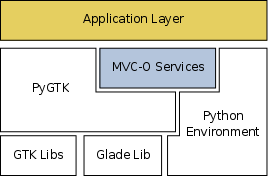
\includegraphics[width=8cm]{figs/png/arch}
\caption{\label{HLA_f}Overview of the architecture}
\end{center}
\end{figure}



In terms of functionalities, at the highest level is located the
\emph{Application Layer}, which is partially based on the \mvco
Infrastructure, and whose implementation depends on the application
semantics. The impact of the framework is intended to be as much
little as possible. 

The \emph{\mvco Services Layer} supplies a quasi-generic platform
which implements the \mvc and the \obs. As the figure \ref{HLA_f}
depicts, the \mvco layer is partially based on \pygtk in order to
provide supports for the view and controller parts. Furthermore, model
part may access \pygtk when using the \mvc provided by \pygtk itself,
like for example \codename{TextBuffer} or \codename{TreeModel}
objects. However in general the model part is indenpended on the
specific graphical toolkit.

Lower layers supply several functionalities concerning the graphical
toolkit (GTK and \glade) and the Scripting Environment (namely
Python).



